% BOTTOM caption
% ------------------------
\begin{figure}[!htbp]
\centering
\vspace{1\baselineskip}
% ------------------------
%
% SIDE caption
% ------------------------
%\begin{SCfigure}[\sidecaptionrelwidth][!htbp]
%\centering
%\vspace{1\baselineskip}
%\includegraphics[width=0.5\textwidth]
% ------------------------
%
% Main information
% ===========================================================
\begin{subfigure}{0.45\textwidth}
	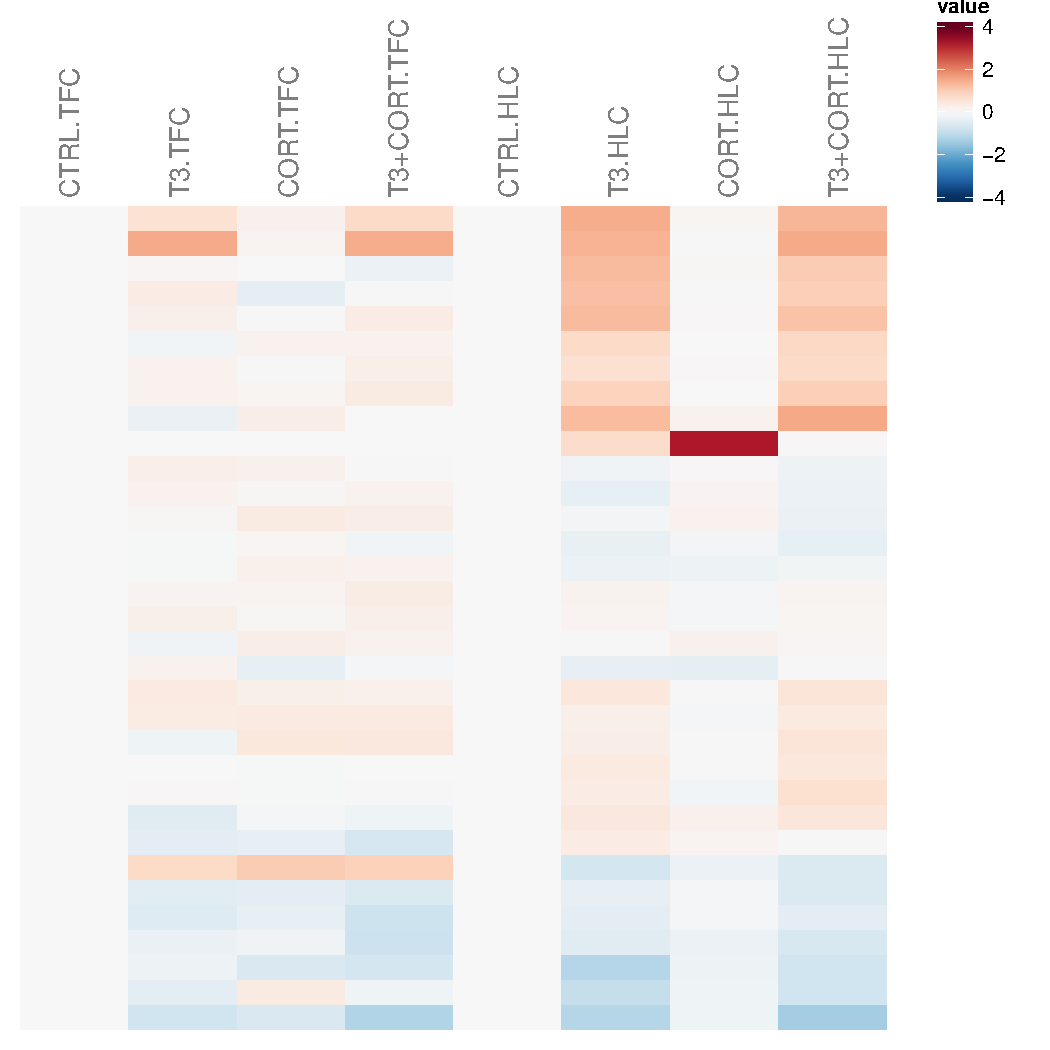
\includegraphics[width=\textwidth]
	{Figures/comparison-tfc-hlc-medna/comparison-tfc-hlc-medna-all.pdf}
	\caption{}
	\label{subfig:comparison-tfc-hlc-medna-all}
\end{subfigure}
~
\begin{subfigure}{0.45\textwidth}
	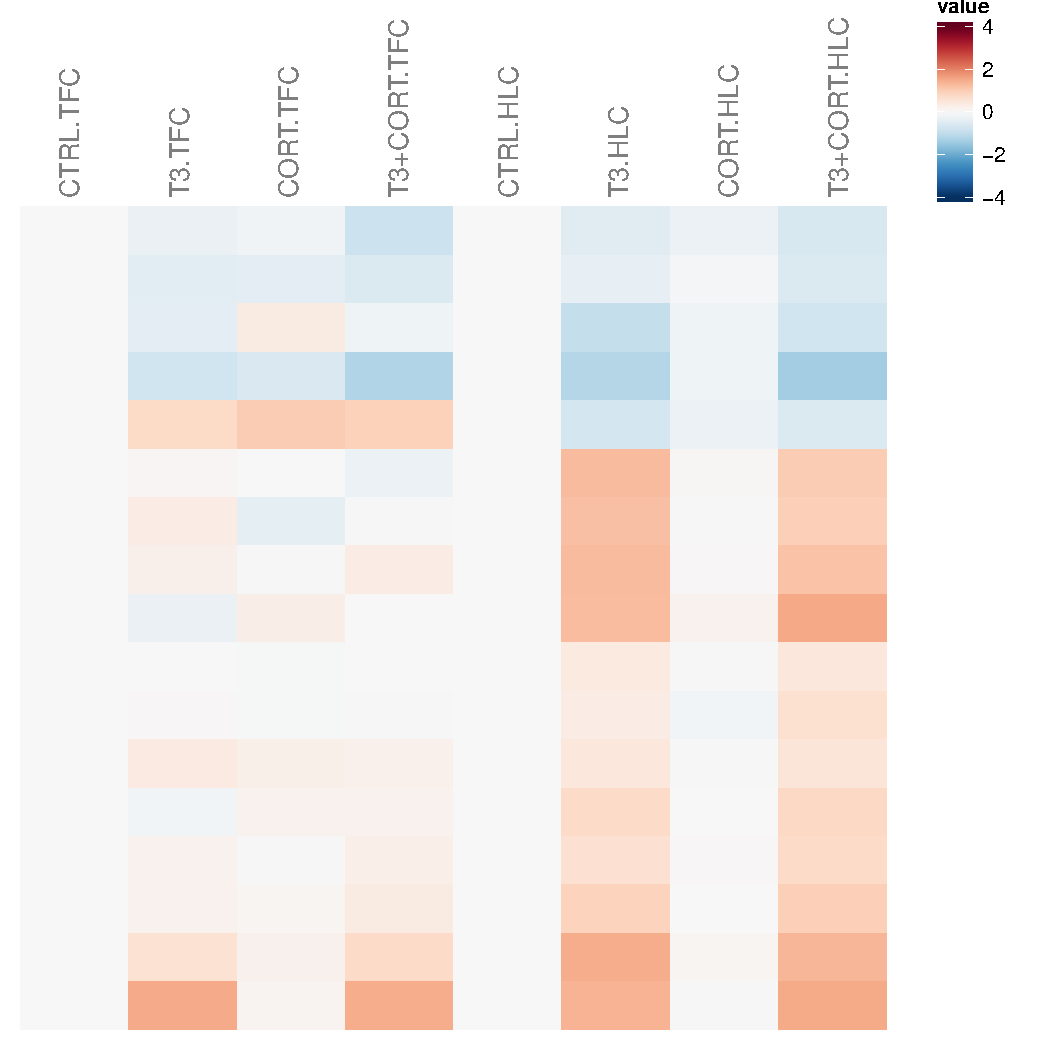
\includegraphics[width=\textwidth]
	{Figures/comparison-tfc-hlc-medna/comparison-tfc-hlc-medna-de.pdf}
	\caption{}
	\label{subfig:comparison-tfc-hlc-medna-de}
\end{subfigure}
\caption[Profils d'expression des gènes impliqués dans la méthylation de l'ADN]
{
Comparaison des profils d'expression, dans l'épiderme caudal et les bourgeons de membres postérieurs, des gènes impliqués dans la méthylation de l'\gls{dna}
\ref{subfig:comparison-tfc-hlc-medna-all} Tous les gènes.
\ref{subfig:comparison-tfc-hlc-medna-de} Sélection des gènes différentiellement exprimés dans au moins une condition.
}
\label{fig:comparison-tfc-hlc-medna}
% ===========================================================
%
% BOTTOM caption
% ------------------------
\end{figure}
% ------------------------
%
% SIDE caption
% ------------------------
%\end{SCfigure}
% ------------------------